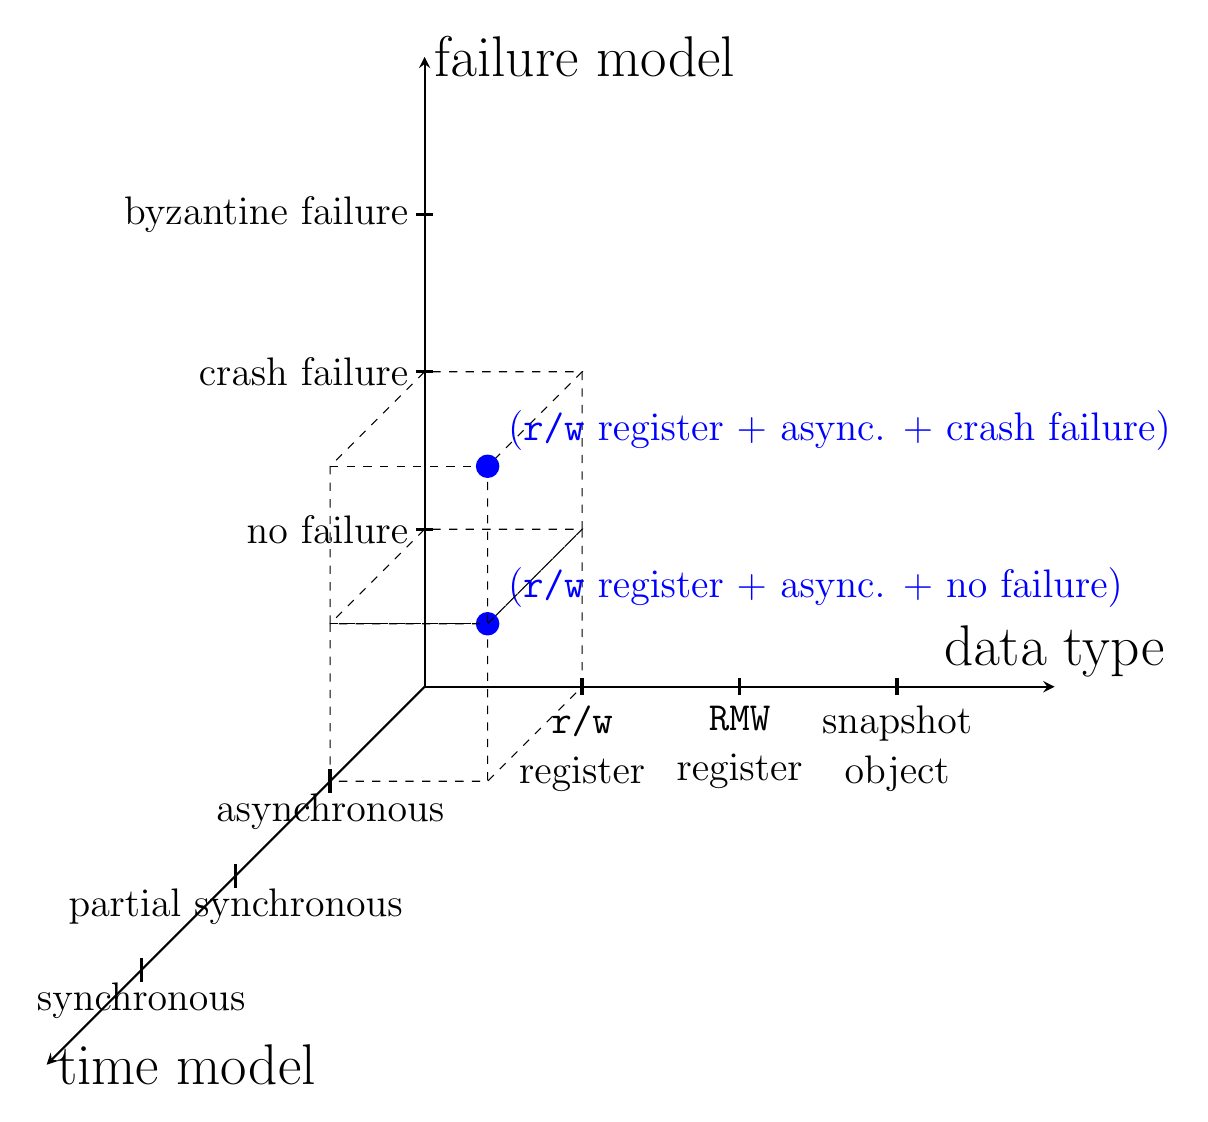
\begin{tikzpicture}[x = 0.5cm, y = 0.5cm, z = 0.3cm, >=stealth, font = \Large]
% The axes
\draw[->, thick] (xyz cs:x=0) -- (xyz cs:x = 16) node[above, font = \huge] {$\textrm{data type}$};
\draw[->, thick] (xyz cs:y=0) -- (xyz cs:y = 16) node[right, font = \huge] {$\textrm{failure model}$};
\draw[->, thick] (xyz cs:z=0) -- (xyz cs:z = -16) node[right, font = \huge] {$\textrm{time model}$};
% The thin ticks
% \foreach \coo in {-13,-12,...,13}
% {
%   \draw (\coo,-1.5pt) -- (\coo,1.5pt);
%   \draw (-1.5pt,\coo) -- (1.5pt,\coo);
%   \draw (xyz cs:y=-0.15pt,z=\coo) -- (xyz cs:y=0.15pt,z=\coo);
% }

% \draw () to ();
% The thick ticks

% ticks for data types
\draw[very thick] (4,-3pt) -- (4,3pt) node[below = 6pt, align = center] {\texttt{r/w} \\ register};
\draw[very thick] (8,-3pt) -- (8,3pt) node[below = 6pt, align = center] {\texttt{RMW} \\ register};
\draw[very thick] (12,-3pt) -- (12,3pt) node[below = 6pt, align = center] {snapshot \\ object};

% ticks for failure models
\draw[very thick] (-3pt,4) -- (3pt,4) node[left = 5pt] {no failure};
\draw[very thick] (-3pt,8) -- (3pt,8) node[left = 5pt] {crash failure};
\draw[very thick] (-3pt,12) -- (3pt,12) node[left = 5pt] {byzantine failure};

% ticks for time models
\draw[very thick] (xyz cs:y=-0.3pt,z=-4) -- (xyz cs:y=0.3pt,z=-4) node[below = 5pt] {asynchronous};
\draw[very thick] (xyz cs:y=-0.3pt,z=-8) -- (xyz cs:y=0.3pt,z=-8) node[below = 5pt] {partial synchronous};
\draw[very thick] (xyz cs:y=-0.3pt,z=-12) -- (xyz cs:y=0.3pt,z=-12) node[below = 5pt] {synchronous};

\uncover<2->
{
% for the case: \texttt{r/w} register + async. + no failure)
\begin{scope}[]
\draw[dashed] 
  (xyz cs:z = -4) coordinate (z) -- 
  +(0,4) coordinate (yz) -- 
  (xyz cs:y = 4) coordinate (y) -- 
  +(4,0) coordinate (xy)-- 
  ++(xyz cs:x = 4, z = -4) coordinate (xyz) --
  +(0,-4) coordinate (w) --
  cycle;
\draw[dashed] (yz) -- (xyz);
\draw[dashed] (xy) |- (4,0) -- (w);

% Dots and labels for P, Q
\node[fill = blue, circle, inner sep = 3pt, label = {[above right, blue, font = \Large] 30: (\texttt{r/w} register + async. + no failure)}] at (xyz) {};
\end{scope}

% for the case: \texttt{r/w} register + async. + crash failure)
\begin{scope}[yshift = 2cm]
\draw[dashed] 
  (xyz cs:z = -4) coordinate (z) -- 
  +(0,4) coordinate (yz) -- 
  (xyz cs:y = 4) coordinate (y) -- 
  +(4,0) coordinate (xy)-- 
  ++(xyz cs:x = 4, z = -4) coordinate (xyz) --
  +(0,-4) coordinate (w) --
  cycle;
\draw[dashed] (yz) -- (xyz);
\draw[dashed] (xy) |- (4,0) -- (w);

% Dots and labels for P, Q
\node[fill = blue, circle, inner sep = 3pt, label = {[above right, blue, font = \Large] 30: (\texttt{r/w} register + async. + crash failure)}] at (xyz) {};
\end{scope}
}

% \node[fill = blue, circle, inner sep = 3pt, label = {[above] 90: $w$}] at (w) {};
% \node[fill = blue, circle, inner sep = 3pt, label = {[above] 90: $xy$}] at (xy) {};
% \node[fill = blue, circle, inner sep = 3pt, label = {[above] 90: $z$}] at (z) {};
% \node[fill = blue, circle, inner sep = 3pt, label = {[above] 90: $yz$}] at (yz) {};
% \node[fill = blue, circle, inner sep = 3pt, label = {[above] 90: $y$}] at (y) {};
% \node[fill,circle,inner sep=1.5pt,label={above:$P(3,0,5)$}] at (3,5) {};
% The origin
% \node[align=center] at (3,-3) (ori) {(0,0,0)\\\text{origin}};
% \draw[->,help lines,shorten >=3pt] (ori) .. controls (1,-2) and (1.2,-1.5) .. (0,0,0);
\end{tikzpicture}